\documentclass[11pt, a4paper]{article}

\usepackage{graphicx}
\usepackage[english]{babel}
\usepackage[utf8x]{inputenc}
\usepackage{amsmath}
\usepackage{subfig}

\usepackage[a4paper,top=3cm,bottom=2cm,left=2cm,right=2cm,marginparwidth=1.75cm]{geometry}
\graphicspath{ {./images} }

\makeatletter
\renewcommand*\env@matrix[1][*\c@MaxMatrixCols c]{%
  \hskip -\arraycolsep
  \let\@ifnextchar\new@ifnextchar
  \array{#1}}
\makeatother


\begin{document}

\setcounter{section}{7}
\section{Lecture 8 (05/03/2020)}
\subsection{Angular momentum}
Imagine a mass on a table that is connected to the middle of the table with a cable. 
This mass is rotating on the table. Figure 1 (a) and (b) contain the top and isometric view of this 
situation.

\begin{figure}[h]
  \centering
  \subfloat[Isometric]{{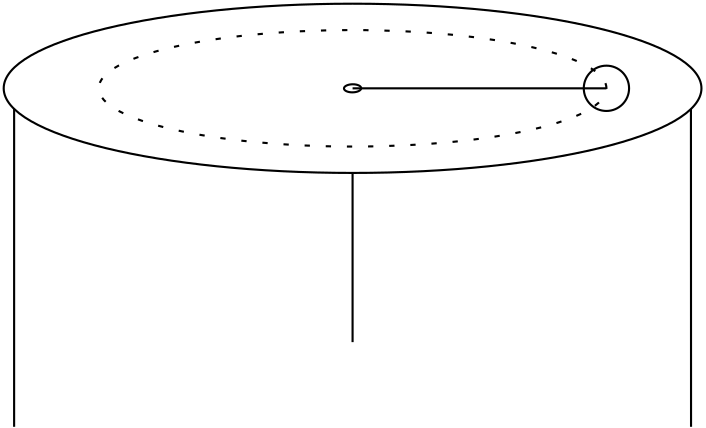
\includegraphics[width=50mm]{images/Angular_momentum_iso.png}}}%
  \qquad
  \subfloat[Top]{{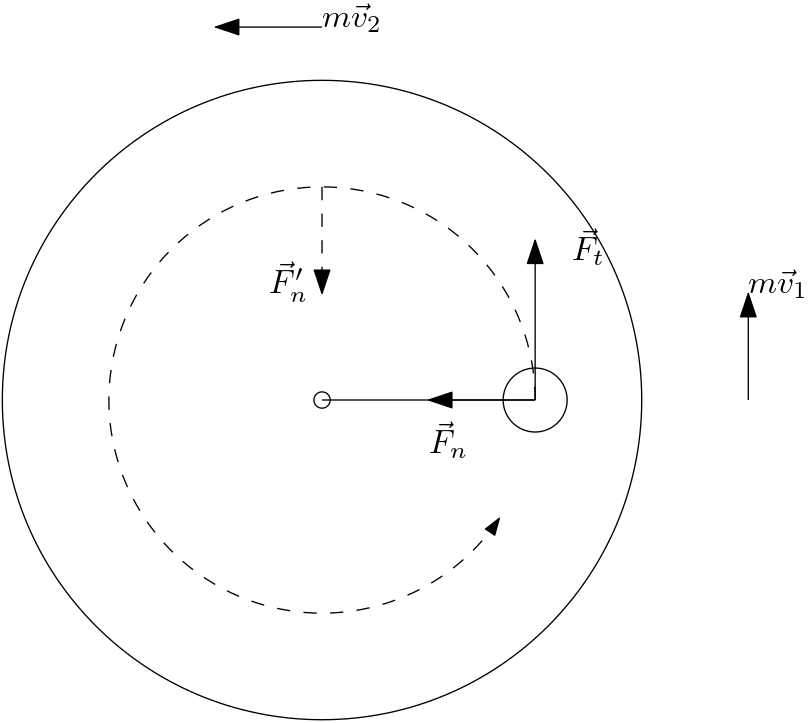
\includegraphics[width=50mm]{images/Angular_momentum_top.png}}}%
  \caption{The situation of the mass rotating on the table}
\end{figure}

This figure leads to the following question: Does conservation of momentum apply to this situation? 
Recall that conservation of momentum looks like the following if described mathematically:
\begin{equation}
    \int_{t_1}^{t_2} \vec{F}\,dt = m\vec{v}_2 - m\vec{v}_1 = 0
\end{equation}

If we look at the Free Body Diagram of the rotating mass we will see that the direction of the forces 
changes relative to time. This means that the direction of the momentum changes. Since momentum is a 
vector, a change in direction also implies a change in momentum even if the magnitude of the momentum 
stays the same. Because of this we instead look at the moment:
\begin{gather}
    \vec{M} = \vec{r} \times \vec{F}\\
    \int_{t_1}^{t_2} \vec{r} \times \vec{F}\,dt = \vec{r}\times m\vec{v}_2 - \vec{r}\times m\vec{v}_1
\end{gather}
The integral $\int \vec{r} \times \vec{F}\,dt$ is referred to as angular impulse (stootmoment in het 
Nederlands) and the term $\vec{r}\times m\vec{v}_2 - \vec{r}\times m\vec{v}_1$ is referred to as angular
momentum (impulsmoment in het Nederlands). Looking at equation (2) and noting that the resulting moment 
should be 0 since the forces passes through the center of rotation, we can colclude the following:
\begin{equation}
    \int \vec{r} \times \vec{F}\,dt = 0
\end{equation}
Hence angular momentum is conserved.

\subsection{Steady fluid flow}
Recall Newton's formulation of his second law:
\begin{equation}
    \Sigma \vec{F} = \frac{d(m\vec{v})}{dt}
\end{equation}
if the flow is considered to be a steady flow we know that the velocity does in fact not change. 
This takes the following form:
\begin{equation}
    \Sigma \vec{F} = \vec{v}_2 \cdot \frac{dm}{dt} -  \vec{v}_1 \cdot \frac{dm}{dt}
\end{equation}
Since we consider a flow through a pipe we know that the fluid going out is the same as the amount
of fluid going in, thus the flow through the pipe is described as an input of $dm$ and an output of
the same amount of mass $dm$. See also figure 3.

\begin{figure}[h]
  \centerline{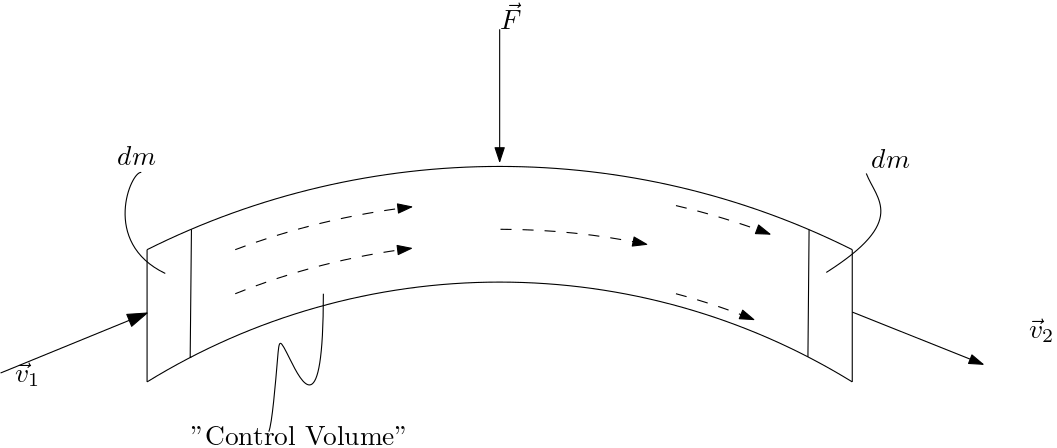
\includegraphics[width=100mm]{images/Fluid_flow.png}}
  \caption{Steady flow of a fluid in a pipe}
\end{figure}

The control volume can be considered as an amount of momentum going in and an amount of momentum going out.
This implies that a force is required to keep a pipe in place if a fluid is flowing through a pipe. 
The resulting force $\vec{F}$ from equation (6) represents the amount of force needed to keep the pipe 
in place. This subject will be discussed in much greater detail in a later course\footnote{WB1530-14, Thermofluids, TU Delft}.

\end{document}
